% Template for Cogsci submission with R Markdown

% Stuff changed from original Markdown PLOS Template
\documentclass[10pt, letterpaper]{article}

\usepackage{cogsci}
\usepackage{pslatex}
\usepackage{float}
\usepackage{caption}

% amsmath package, useful for mathematical formulas
\usepackage{amsmath}

% amssymb package, useful for mathematical symbols
\usepackage{amssymb}

% hyperref package, useful for hyperlinks
\usepackage{hyperref}

% graphicx package, useful for including eps and pdf graphics
% include graphics with the command \includegraphics
\usepackage{graphicx}

% Sweave(-like)
\usepackage{fancyvrb}
\DefineVerbatimEnvironment{Sinput}{Verbatim}{fontshape=sl}
\DefineVerbatimEnvironment{Soutput}{Verbatim}{}
\DefineVerbatimEnvironment{Scode}{Verbatim}{fontshape=sl}
\newenvironment{Schunk}{}{}
\DefineVerbatimEnvironment{Code}{Verbatim}{}
\DefineVerbatimEnvironment{CodeInput}{Verbatim}{fontshape=sl}
\DefineVerbatimEnvironment{CodeOutput}{Verbatim}{}
\newenvironment{CodeChunk}{}{}

% cite package, to clean up citations in the main text. Do not remove.
\usepackage{apacite}

% KM added 1/4/18 to allow control of blind submission


\usepackage{color}

% Use doublespacing - comment out for single spacing
%\usepackage{setspace}
%\doublespacing


% % Text layout
% \topmargin 0.0cm
% \oddsidemargin 0.5cm
% \evensidemargin 0.5cm
% \textwidth 16cm
% \textheight 21cm

\title{Re-examining cross-cultural similarity judgments using lexical
co-occurrence}

\usepackage[utf8]{inputenc}
\usepackage[T1, T2A, T5]{fontenc}
\usepackage{kotex}
\usepackage{booktabs}
\usepackage{longtable}
\usepackage{array}
\usepackage{multirow}
\usepackage{wrapfig}
\usepackage{float}
\usepackage{colortbl}
\usepackage{pdflscape}
\usepackage{tabu}
\usepackage{threeparttable}
\usepackage{threeparttablex}
\usepackage[normalem]{ulem}
\usepackage{makecell}
\usepackage{xcolor}

\author{{\large \bf Khuyen N. Le (knl005@ucsd.edu)}$^{1}$, {\large \bf Alexandra Carstensen (abc@ucsd.edu)}$^{1}$, \\ {\large \bf Shan Gao (shangaocog@gmail.com)$^2$}, {\large \bf Michael C. Frank (mcfrank@stanford.edu)$^3$},  \AND $^1$Department of Psychology, University of California, San Diego, $^2$Department of Psychology, University of Chicago, \\ $^3$Department of Psychology, Stanford University }

\newlength{\cslhangindent}
\setlength{\cslhangindent}{1.5em}
\newenvironment{CSLReferences}%
  {}%
  {\par}

\begin{document}

\maketitle

\begin{abstract}
Is ``cow'' more closely related to ``grass'' or ``chicken''? Speakers of
different languages judge similarity in this context differently, but
why? One possibility is that cultures co-varying with these languages
induce differences in conceptualizations of similarity. Specifically,
East Asian cultures may promote reasoning about thematic similarity, by
which cow and grass are more related, whereas Western cultures may bias
judgments toward taxonomic relations, like cow-chicken. This difference
in notions of similarity is the consensus interpretation for
cross-cultural variation in this paradigm. We consider, and provide
evidence for, an alternative possibility, by which notions of similarity
are similar across contexts, but the statistics of the environment vary.
On this account, similarity judgments are guided by co-occurrence in
experience, and hearing about cows and grass or cows and chickens more
often could induce preferences for these groupings, and account in part
for apparent differences in notions of similarity across contexts.

\textbf{Keywords:}
similarity; culture; language; semantics; lexical co-occurrence;
variation; US; China; Vietnam
\end{abstract}

\hypertarget{introduction}{%
\section{Introduction}\label{introduction}}

Many cognitive processes rely on similarity, from inference and
generalization to analogy, mathematics, and science. There is
substantial consistency in human similarity reasoning, but also
systematic variation across cultural and linguistic contexts. In
particular, there is considerable evidence showing that similarity
reasoning in East Asian cultural contexts differs from that in Western
cultures (e.g. Nisbett \& Masada, 2003). For example, in a triad task
comparing preferences for taxonomic and thematic similarity (choose two
out of three words that are most related to one another), Ji, Zhang, \&
Nisbett (2004) found that Chinese participants preferred thematic
matching to a greater extent than European Americans. In an image
version of this task, Chinese children (9-10 years old) are also more
likely to choose thematic matches compared to their American
counterparts (Chiu, 1972). This cross-cultural difference is also
observed in novel object categorization, with Chinese participants
preferring to group by family resemblance across multiple features and
Americans preferring a single-feature rule (Norenzayan, Smith, Kim, \&
Nisbett, 2002). Across tasks, East Asian participants show a preference
for thematic similarity based on causal, spatial, and temporal
relationships while Western participants are more likely to make
taxonomic matches based on the similarity of attributes, like shared
color or shape, among objects (see Markman \& Hutchinson, 1984 for a
discussion of these types of similarity).

An influential perspective within cultural psychology links these
differences in similarity judgment to tendencies toward analytic
processing in Western cultures, and holistic processing in East Asian
cultures (Nisbett, 2003). Analytic processing emphasizes rule-like
relationships predicated on objects and their properties and,
correspondingly, taxonomic similarity, while holistic processing
emphasizes relations between objects and their context and therefor,
thematic similarity. In related work, East Asian participants show a
higher level of sensitivity to context than their Western counterparts
when reproducing drawings from memory (Ji, Peng, \& Nisbett, 2000);
visually exploring naturalistic scenes (Chua, Boland, \& Nisbett, 2005);
describing scenes (Masuda \& Nisbett, 2001); and in explaining the
causes of ambiguous behaviors (Choi, Nisbett, \& Norenzayan, 1999). The
consensus interpretation in this literature ascribes cross-cultural
differences in similarity judgment to variation in the
\emph{conceptualization} of similarity -- with people from East Asian
cultures relying on a more thematic notion of similarity than
Westerners.

Alternatively, these judgments could be shaped by cross-cultural
differences in the \emph{input} to similarity judgment, that is, the
statistics of the environment, and the content of everyday experiences.
Perhaps when faced with the triad task, participants from all cultures
follow the same process for conceptualizing similarity, but rely on
language or culture-specific input to this process. If we observe a
difference in categorization between East Asian and Western
participants, it could be that members of both groups use the same
procedure (considering similarity that is influenced by both taxonomic
and thematic relations), but the input to this procedure differ between
cultures, with East Asian participants exposed to more support for
thematic similarity in the language they hear in comparison to their
Western counterparts. We might also expect that both conceptualization
of similarity and input from experience play a role in driving
cross-cultural differences -- East Asian participants may be exposed to
more instances of thematic similarity, and prefer to conceptualize
similarity as thematic to a greater extent than Westerners.

\hypertarget{estimating-variation-in-experience-via-language-statistics}{%
\subsection{Estimating variation in experience via language
statistics}\label{estimating-variation-in-experience-via-language-statistics}}

To determine whether varied input to similarity judgments can in part
explain cross-cultural differences, we need a way to operationalize
variation in exposure to thematic and taxonomic relations. While
exposure to types of similarity is difficult to measure, the statistics
of language can provide a rough proxy. Language statistics are useful in
that they are part of the input to everyday experience -- and indeed,
may afford many of the `experiences' that people have with infrequently
encountered items, like cows or helicopters -- and they provide an
accessible measure. Previous work also suggests that language
statistics, such as lexical co-occurrence or cosine distance of word
embeddings, can be good predictors of similarity reasoning. Semantic
models that are constructed using lexical co-occurrence (in comparison
to annotated relations) have been shown to perform well on predicting
human judgments about similarity between word pairs that are
thematically or taxonomically related (Rohde, Gonnerman, \& Plaut,
2006). Relatedly, a model trained on word-document co-occurrence can
predict word association and the effects of semantic association on a
variety of linguistic tasks (Griffiths, Steyvers, \& Tenenbaum, 2007).
Word embeddings like word2vec, gloVe, and fastText have also been shown
to be good predictors for similarity judgments Jatnika, Bijaksana, \&
Suryani (2019).

Our study uses cosine distances of fastText word vectors as a measure of
lexical co-occurrence\footnote{We also carried out our analysis using
  raw lexical co-occurrences and obtained similar results.}. fastText is
a system that uses lexical co-occurrence information to generate a
vector representing each word in its lexicon (Mikolov, Grave,
Bojanowski, Puhrsch, \& Joulin, 2018). fastText has also been shown to
be sensitive to cultural differences in word meanings: Thompson \&
Lupyan (2020) demonstrated that the distribution of semantic meaning
clusters generated by fastText trained on language-specific corpora
correlates with the cultural, historical, and geographical similarities
of these languages.

We note that language statistics may incorporate both cultural-specific
environmental statistics, that is, the experiential \emph{input} to
similarity judgments, and culture-specific senses of similarity, the
\emph{conceptualization} of similarity. For example, cultural features
(like farming) can lead to differences in environmental statistics
(seeing cows and grass) and these can influence language (talking more
about cows and grass). But other cultural features (like conceiving of
similarity thematically) could also cause individuals to talk
differently about the same experiences (mentioning what cows eat rather
than what other animals cows are like). Acoordingly, our approach
examines the extent to which language statistics can predict
cross-cultural differences in similarity judgments with the
understanding that language statistics are likely a proxy for both
\emph{input} to and \emph{conceptualization} of similarity.

\hypertarget{the-present-study}{%
\subsection{The present study}\label{the-present-study}}

The present study tests whether the statistics of language can be used
to predict cross-cultural differences in similarity judgments, and
particularly, whether this approach provides additional insight beyond
cross-cultural characterizations based on taxonomic vs thematic
preferences.

We measured taxonomic versus thematic similarity matching in a
forced-choice word triad task in three populations. Following Ji et al.
(2004), we measured preferences in the US and China. In addition, we
collected data in a novel context: Vietnam. Vietnam is a Southeast Asian
country that borders China and has historically been greatly influenced
by Chinese culture (Hui, 2002). Therefore, it serves as a suitable
cultural context to investigate whether the claim made by Ji et al.
(2004) and previous studies -- that Eastern and Western cultures have
different notions of similarity -- extends beyond mainland China. In
addition to these replication and extension questions, we tested whether
fastText vectors from corpora corresponding to each language context
(English, Mandarin, and Vietnamese) are good predictors for similarity
judgments in each population.

This study is correlational and cannot evaluate causal relationships
between environmental statistics and similarity judgments. However, this
work can inform potential mechanisms by examining whether similarity
judgments covary with environmental statistics that differ across these
contexts. Our specific research questions are as follows:~

\begin{enumerate}
\def\labelenumi{\arabic{enumi}.}
\item
  Do we replicate cross-cultural differences in similarity judgments
  between East Asian and Western cultures?
\item
  Are these cross-cultural differences related to differences in
  language?
\item
  Is our language model specific to items with a taxonomic-thematic
  contrast, or can it predict similarity more generally?~
\end{enumerate}

To preview our results, we replicate US-China differences and find that
Vietnamese judgments are intermediate between these two. We find that
language-specific statistics provide good predictions for cross-cultural
differences in similarity judgments, and additionally, for more general
similarity judgments that do not contrast taxonomic and thematic
matches. Critically, the stimuli used to assess this more general case
of similarity reasoning were constructed to be outside the scope of
explanation for taxonomic-thematic accounts (for use as filler items).
While the language model may succeed in taxonomic-thematic similarity
predictions by picking up on differences in the \emph{conceptualization}
of similarity that are reflected in language data, this
conceptualization account provides no prediction for these filler
stimuli. Accordingly, these filler stimuli provide the strongest test of
the language model, demonstrating that it can explain variation in
similarity judgments beyond that explained by thematic or taxonomic
conceptualizations of similarity. Taken together, our findings provide
support for an alternative to previous accounts, on which differing
cultures induce differing conceptions of similarity. They show that
language can account for culture-specific variation in similarity
reasoning, both for taxonomic-thematic judgments and for judgments not
attributable to these senses of similarity. While these findings do not
rule out contributions from differing senses of similarity, they show it
is possible to explain cross-cultural differences in similarity
judgments without invoking variation in notions of similarity, at least
in some cases.

\hypertarget{methods}{%
\section{Methods}\label{methods}}

\hypertarget{participants}{%
\subsection{Participants}\label{participants}}

We recruited 200 participants from the US, 199 participants from
Vietnam, and 200 participants from mainland China. US participants were
recruited through snowball sampling seeded with Stanford student email
lists, Vietnam participants were recruited through snowball sampling
seeded with Vietnam-based student groups on Facebook, and mainland China
participants were recruited through snowball sampling seeded with group
chats on WeChat. US participants were compensated with \$5 gift
certificates (USD), VN participants received 50,000₫ (VND) in phone
credit, and mainland China participants received 25CNY through WeChat
credit transfer.

We excluded 8 US participants, 62 Vietnam participants, and 16 China
participants who missed 2 or more attention checks. We followed 4
exclusion criteria that aim to retain only participants who are
influenced by one culture: (1) non-native speakers of English and
Vietnamese, respectively, (2) fluent in at least one of the other two
study languages (Vietnamese for US participants, English for Vietnamese
participants and Chinese participants), (3) have lived outside of the
test country (US, Vietnam, or China) for more than two years, and (4)
have significant international experience (more than 6 international
experiences of 2 days or longer.) We did not use a particular criterion
for a language if it would exclude 25\% or more of any one sample. In
this round of exclusion, we excluded 73 US, 27 Vietnam participants, and
35 China participants. After these exclusions, the US sample included
119 participants (30M, 84F, 3 non-binary, 2 other), with mean age = 22.2
(SD = 8.15) and median age = 20. The Vietnam sample included 110
participants (34M, 71F, 5 other), with mean age = 22.21 (SD = 5.81) and
median age = 21. The China sample included 149 participants (61M, 87F, 1
other), with mean age = 23.1 (SD = 3.65) and median age = 23.\footnote{A
  table summarizing number of participants lost at each round of
  exclusions is included in the Supplementary Information.}

We preregistered a more stringent exclusion criterion where participants
were excluded if they missed any attention checks. However, this led to
a small sample size, especially for Vietnam context (US = 109, China =
132, Vietnam = 57). Our reported results with the less stringent
exclusion criterion (detailed above) is largely not different from the
results with the preregistered criterion. Any differences are noted in
the Results \& Discussion section.

\hypertarget{stimuli-materials}{%
\subsection{Stimuli Materials}\label{stimuli-materials}}

We adapted stimuli from previous studies to create a set of test triads
consisting of a cue, with one thematic and one taxonomic match option.
For example, ``cow,'' ``grass,'' and ``chicken,'' where ``cow'' is the
cue, ``grass'' is the thematic match, and ``chicken'' the taxonomic
match. We included 105 such triads, a superset including triads pulled
from supplemental information and in-text examples across the
literature, and others that we adapted or created . We selected triads
on the basis of cultural familiarity in the US, Vietnam, and China. The
triads were originally in English; they were translated to Vietnamese
and Mandarin by a fluent bilingual speaker in each language. The
translations were then checked for accuracy after backtranslation to
English by another fluent bilingual in each language who was naive to
the original English versions. All materials are available at {[}BLINDED
FOR REVIEW{]}.

\hypertarget{procedure}{%
\subsection{Procedure}\label{procedure}}

Each participant completed all 105 triads in sets of 21 trials at a time
(10 test triads, 10 filler triads, and 1 attention check per page), by
selecting the match most related to the cue (``Which thing is most
closely related to the bolded item?'' and translated equivalents). The
test triads were presented with 105 filler triads mixed in, to obscure
the taxonomic-thematic two-answer forced choice structure of the test
stimuli and reduce the likelihood that participants would become aware
of the design. The filler triads were groups of three semantically
related words, but where the match options were not distinguished by
thematic vs.~taxonomic similarity, e.g., cue ``bird'' with match options
``lizard'' and ``toad.'' Additionally, we included 10 attention check
trials, which were formatted like the test and filler triads but
included an instruction instead of a cue item, e.g., ``Choose wife''
with match options ``wife'' and ``husband.'' In total, each participant
completed 210 similarity judgments and 10 attention check questions,
with triads presented in randomized orders that varied between subjects.

\hypertarget{corpus-model}{%
\subsection{Corpus model}\label{corpus-model}}

Our general approach is to predict behavioral preferences in similarity
judgment using relative similarity between word embeddings.

\hypertarget{word-vector-retrieval}{%
\paragraph{Word vector retrieval}\label{word-vector-retrieval}}

We use the fastText pre-trained models of English, Mandarin, and
Vietnamese in Grave, Bojanowski, Gupta, Joulin, \& Mikolov (2018). These
models are trained on Common Crawl and Wikipedia using We distribute
pre-trained word vectors for 157 languages, trained on Common Crawl and
Wikipedia using fastText. These models were trained using a Continuous
Bag of Words (CBOW) with position-weights and a window of size 5. The
models use character n-grams of length 5 and 10 negative examples. From
the aforementioned models, we retrieve the word vectors (dimension 300)
for each word we are interested in.

\hypertarget{similarity-model}{%
\paragraph{Similarity model}\label{similarity-model}}

To give an intuition for our model, consider again the cow-grass-chicken
triad: we retrieved word vectors for ``cow'' and ``grass'', and
calculate the cosine distance between these vectors. Similarly, we
retrieved vectors for ``cow'' and ``chicken'' and calculate the cosine
distance between them. Our similarity prediction is then inversely
proportional to the ratio of cosine distance of these pairs. This is
because a larger cosine distance means the word vectors are further
apart, and thus the words are less similar. For example, if the cosine
distance of thematic cow-grass is 0.7 and the cosine distance of
taxonomic cow-chicken is 0.3, then our model predicts, correspondingly,
that 30\% of responses to the triad will be grass, and the other 70\%
chicken.

In practice, we calculated the cosine distance between each cue-thematic
match (thematic cosine distance) and cue-taxonomic match (taxonomic
cosine distance), using the spatial.distance.cosine function from the
SciPy package (Virtanen et al., 2020). We then calculated the thematic
cosine distance proportion as thematic cosine distance over the sum of
taxonomic cosine distance and thematic cosine distance. We did this for
all three corpora. We were able to obtain predictions for all triads in
all languages. We then use a mixed-effects regression to evaluate how
well each corpus model predicts participants' similarity judgments,
across triads and cultural contexts. All analyses are available at
{[}BLINDED FOR REVIEW{]}.

\hypertarget{results-discussion}{%
\section{Results \& Discussion}\label{results-discussion}}

\hypertarget{replication-of-previous-work-and-extension-to-a-vietnamese-sample}{%
\subsection{1. Replication of previous work and extension to a
Vietnamese
sample}\label{replication-of-previous-work-and-extension-to-a-vietnamese-sample}}

Following previous work, we would expect participants from mainland
China to prefer thematic matches more than US participants (to use the
cow-grass-chicken triad: we would expect participants from mainland
China to prefer the cow-grass match over the cow-chicken match to a
larger extent compared to US participants). We would also expect that
participants from Vietnam would pattern with China, and also show a
significantly higher preference for thematic matches compare to US
participants.

The group means of proportion of thematic response in mainland China is
the highest (M = 0.65, SD = 0.11), followed by the groups means in
Vietnam (M = 0.6, SD = 0.11), which is slightly higher than that of the
US (M = 0.56, SD = 0.17) (Figure 1).

\begin{CodeChunk}
\begin{figure}[tb]

{\centering 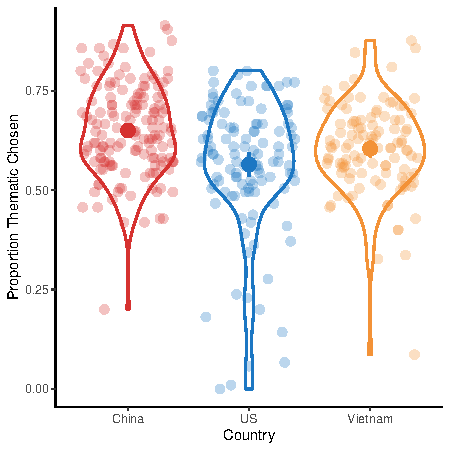
\includegraphics{figs/unnamed-chunk-1-1} 

}

\caption[Proportion of thematic responses by country]{Proportion of thematic responses by country.}\label{fig:unnamed-chunk-1}
\end{figure}
\end{CodeChunk}

To test for cross-context differences in similarity judgments between
the countries, we ran a mixed-effects logistic regression predicting
triad responding (taxonomic or thematic) with country (US, China, or
Vietnam) as a fixed effect. As random effects, we included an intercept
per subject and one per triad, as well as by-triad random slopes for
country to account for variation in the country effect across triads.

Overall, there is a significant effect of country on proportion of
thematic responses (\(\chi^2\)(2) = 15.37, p \textless{} .001). However,
this effect is driven by the difference between US and China responding
(\(\beta\) = -0.48, p \textless{} .001). There is no statistical
difference between the Vietnam and China responding (\(\beta\) = -0.22,
p = 0.09), and the US and Vietnam responding (\(\beta\) = 0.26, p =
0.086).

On this analysis, we do not find support that the US-China tendencies
toward taxonomic and thematic responding (respectively) extend to the
US-Vietnam comparison. Accordingly, we cannot speak to overall biases
toward thematic responding across Asian cultural contexts broadly, but
we do replicate the differences documented by Ji et al. (2004) between
the US and China. However, in our corpus model comparison, we do find
evidence for different, more fine-grained variation in similarity
judgments between the US and Vietnam.

\hypertarget{language-statistics-as-a-predictor-for-cross-cultural-variation-in-similarity-judgments}{%
\subsection{2. Language statistics as a predictor for cross-cultural
variation in similarity
judgments}\label{language-statistics-as-a-predictor-for-cross-cultural-variation-in-similarity-judgments}}

\hypertarget{single-corpus-model}{%
\subsubsection{Single corpus model}\label{single-corpus-model}}

To test whether variation in language statistics can explain differences
in similarity judgments between US and Vietnam participants, we compare
logistic mixed-effects regression models fit to the thematic responding
data from each country separately. We first ask how well each corpus
model (English, Vietnamese, or Mandarin) predicts similarity judgments
by speakers of the corresponding language (US, Vietnam, or China). To do
this, we use a mixed-effects logistic regression to predict triad
responses (0=taxonomic or 1=thematic) with corpus prediction (proportion
of cosine distance) as a fixed effect and participant and triad as
random effects. If environmental statistics (as proxied by language
statistics) contribute to the differences in similarity judgments, we
would expect each language corpus to be a good predictor for similarity
judgment responding in its corresponding context.

We found that all corpora are significant predictors of all cultural
context responding, with p \textless{} 0.05 and \(\beta\) from -8.69 to
-2.4. (For a full report, see Supplementary Information.)

While each corpus is a good predictor for its corresponding context, the
fact that all corpora covary with all cultural contexts suggests that
language is such a rich proxy of human experience that even using the
wrong proxy (e.g.~Mandarin for US responding) is informative. A single
corpus model might therefore not be informative in culture-specific
ways, but might only reflect consistency in experiences across cultures.

\hypertarget{multiple-corpora-model}{%
\subsubsection{Multiple corpora model}\label{multiple-corpora-model}}

If language statistics is able to predict meaningful culture-specific
variation in similarity judgment (rather than just consistency across
cultures), we would expect each corpus to be the best predictor of its
corresponding culture compared to the other two corpora. We directly
compare the corpus models by including both as fixed effects in three
mixed-effect regressions (predicting US, Vietnam and China responding)
with the same random effects as above.

For US responding: only the English (EN) corpus is a significant
predictor\footnote{With preregistered exclusion criterion: only the
  English (EN) and Mandarin (ZH) corpus are significant predictors.}. EN
corpus: \(\beta\) = -6.96, \(\chi^2\)(1) = 16.57, p \textless{} .001. VI
corpus: \(\beta\) = -2.22, \(\chi^2\)(1) = 3.73, p = 0.054. ZH corpus:
\(\beta\) = -3.18, \(\chi^2\)(1) = 3.37, p = 0.066.

For Vietnam responding: only the Vietnamese (VI) and Mandarin (ZH)
corpus are significant predictors\footnote{With preregistered exclusion
  criterion: all three corpora are significant predictors.}. EN corpus:
\(\beta\) = -2.98, \(\chi^2\)(1) = 2.58, p = 0.108. VI corpus: \(\beta\)
= -2.75, \(\chi^2\)(1) = 4.84, p = 0.028. ZH corpus: \(\beta\) = -4.39,
\(\chi^2\)(1) = 5.49, p = 0.019.

For China responding: only the Mandarin (ZH) and English (EN) corpus are
significant predictors. EN corpus: \(\beta\) = -3.32, \(\chi^2\)(1) =
7.18, p = 0.007. VI corpus: \(\beta\) = -1.59, \(\chi^2\)(1) = 3.63, p =
0.057. ZH corpus: \(\beta\) = -5.31, \(\chi^2\)(1) = 17.69, p
\textless{} .001.

We observed some level of language specificity from this analysis. The
English corpus is the best predictor for US responding, and the Mandarin
corpus is the best predictor for China response. While this is not the
case with the Vietnamese corpus and the Vietnam responding, the
Vietnamese corpus is still a significant predictor for the Vietnam
responding (Figure 2). These results strengthens our hypothesis that
variation in inputs to similarity judgment (as proxied by language
statistics) can predict cross-cultural variations of similarity
judgment.

\begin{CodeChunk}
\begin{figure}[tb]

{\centering 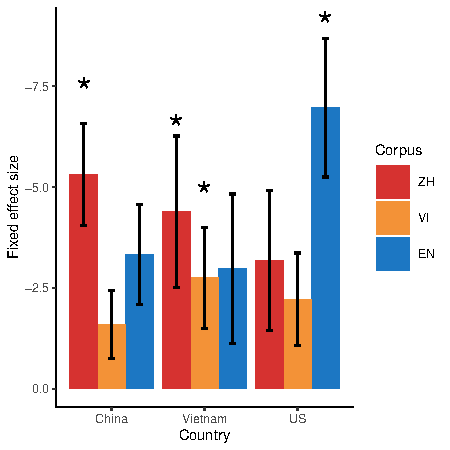
\includegraphics{figs/coeffs_cos-1} 

}

\caption[Fixed effect sizes of each corpus lexical statistics (cosine distance proportion) when included as a predictor for China, Vietnam, and US responding, respectively]{Fixed effect sizes of each corpus lexical statistics (cosine distance proportion) when included as a predictor for China, Vietnam, and US responding, respectively. The English corpus is the best predictor for US response, and the Mandarin corpus is the best predictor for China response.}\label{fig:coeffs_cos}
\end{figure}
\end{CodeChunk}

However, in all cultural contexts, adding the other two corpora produces
a significantly better fit than the identical model without the
additional corpora, and only the corresponding corpus included as a
predictor (US response: \(\chi^2\)(2) = 7.93, p = 0.019; Vietnam
response: \(\chi^2\)(2) = 13.72, p = 0.001; China response:
\(\chi^2\)(2) = 10.56, p = 0.005). This analysis suggests that
culture-specific inputs to similarity judgment (as proxied by language
statistics) do not fully explain cross-cultural differences in
similarity judgment.

\hypertarget{language-statistics-as-a-predictor-for-non-structured-filler-items}{%
\subsection{3. Language statistics as a predictor for non-structured
filler
items}\label{language-statistics-as-a-predictor-for-non-structured-filler-items}}

A possible concern with our approach is that our models using language
statistics in Q2 are only able to account for variation in
thematic/taxonomic preference in similarity judgment because language
statistics is picking up on differences in thematic/taxonomic preference
in conceptualization of similarity. For example, perhaps ``cow'' and
``grass'' co-occurs more than ``cow'' and ``chicken'' in Mandarin
because Chinese speakers prefer thematic relations, and thus talk about
``cow'' and ``grass'' together more often. Vice versa, English speakers
preferring taxonomic relations would talk about ``cow'' and ``chicken''
together more often, hence driving higher lexical co-occurrence for
``cow'' and ``chicken'' in the English corpus. In other words, perhaps
the language statistics models are merely measuring variation in
thematic/taxonomic relation preference in conceptualization of
similarity, only in a different way. If this is the case, language
statistics should not be able to predict responding for filler items
(such as whether ``tomorrow'' or ``yesterday'' is more related to
``today'') because these items do not have a thematic/taxonomic
structure. Additionally, even when one option might be more related to
the cue, such relationship is not systematic throughout the set of
fillers. On the other hand, if language statistics capture similarity
judgment in a more general sense (beyond thematic/taxonomic preference
in conceptualization of similarity), it should also be a significant
predictor for the non-structured filler items.

For each filler triad, we randomly assigned one of the responding
options as `Word1'. Running a mixed-effects logistic regression to
predict responding (Word1 or Word2) with country as the fixed effect and
a random effect structure equivalent to Q1, we found no effect of
country on filler responding (\(\chi^2\)(2) = 0.74, p = 0.692).

Using the same mixed-effects logistic regression structure as the single
corpus models in Q2, we predict responses (1=word1 or 0=word2) of each
cultural context with the corresponding corpus statistics as a fixed
effect, and participant and triad as random effects. We found that in
all cultural contexts, the corresponding corpus is a significant
predictor of responding, with p \textless{} 0.05 and \(\beta\) from
-9.59 to -3.14. (For a full report, see Supplementary Information.)
These results show that the language statistics model is accounting for
general similarity in addition to structured thematic/taxonomic
similarity.

To investigate whether language statistics predicts triads and filler
items differently, we compare the variance in responding that can be
accounted for by language statistics of the corresponding corpus in the
two different types of items (structured triads versus non-structured
filler items). Namely, we ran two mixed-effects logistic regression
models that predict responding across cultural contexts (1=thematic or
word1, 0=taxonomic or word2), with the corresponding corpus statistics
(for e.g., cosine proportion from the English corpus for US responding)
as a fixed effect and participant and item as random effects. Consistent
with our results above, corresponding corpus is a significant predictor
for responding to both triads and filler items (triads: \(\beta\) =
-1.79, \(\chi^2\)(1) = 75.58, p \textless{} .001, fillers: \(\beta\) =
-2, \(\chi^2\)(1) = 70.89, p \textless{} .001). Importantly, we found
comparable conditional \(R^2\) when corresponding corpus is used to
predict only triad items (\(R^2\) = 0.3) and only filler items (\(R^2\)
= 0.26), suggesting that culture-corresponding corpus statistics is able
to explain the same amount of variance in the responding data for either
triads or filler items. This result provides evidence for our view that
language statistics is measuring general tendencies in similarity
judgment, beyond preference for thematic/taxonomic relations.

\hypertarget{general-discussion}{%
\section{General Discussion}\label{general-discussion}}

In this paper, we consider whether statistics of the environment (as
proxied by language statistics) can account for cross-cultural
differences in a classic similarity judgment paradigm, as an alternative
to the view that members of different cultures vary in their
conceptualization of similarity. We replicated the previously documented
contrast between English speakers in the US and Mandarin Chinese
speakers from East Asia (mainland China, Taiwan, Hong Kong, and
Singapore), with mainland China participants preferring thematic
relations to a greater extent compared to US participants. Our sample of
Vietnamese participants showed intermediate response but not
significantly different from either Chinese or US participants. This
finding suggests some limitations on the generality of the cultural
account, which proposes that thematic/taxonomic similarity preference
aligns with East Asian/Western tendency for holistic vs analytic
processing. We found some support for the environmental statistics
account: each corpus statistics is a good predictor for the
corresponding country's similarity judgments, even when other corpus
statistics are included, and even with triads without a
thematic/taxonomic structure. Overall, our results provide evidence that
cross-cultural differences in similarity judgment are related to
linguistic co-occurrence patterns (which also vary across cultures).

There are some important limitations of our approach. While we discuss
cross-cultural variability at the level of countries or larger world
areas, these are not cultural monoliths. For convenience, we
operationalize culture at the level of country, based on where
participants were raised. It is an open question whether performance in
our participant populations (of relatively young and well-educated
adults) is representative of the broader country. This is especially
true for societies with substantial ethnic and cultural variation such
as the US. We expect that our data is likely to underestimate variation
both within and between the countries we sample from.

Additionally, language, culture, cognition, and individual experiences
are intertwined in complex causal relationships. In this study, we
measure language and its relation to cross-cultural differences in
categorization, but these relations test only the plausibility of a
language-based account; they cannot establish the direction of
causality.

Ji et al. (2004) established that culture-aligned differences in this
paradigm exist, even when the test language is held constant, concluding
that ``it is culture (independent of the testing language) that led to
different grouping styles'' in their study. Our data provide a
cautionary note to this conclusion, suggesting that while cultural
differences in similarity judgment exists, we might get better traction
at modelling cross-cultural variation through environmental statistics
such as lexical co-occurrences, rather than treating groups of cultures
as monoliths (East Asian vs Western). However, there are still many open
questions for this account. Our operationalization of environmental
statistics with lexical co-occurrence is a proxy of both language inputs
and culture-specific conceptualization of similarity. The extent to
which cross-cultural differences in similarity judgment are driven by
language versus culture is still an open question. Future work should
also aim to provide a more specific computational account of how lexical
co-occurrence might guide categorization preference beyond the simple
proportion-of-similarity model tested here, and investigate other
individual- or triad-specific factors that might influence how
environmental statistics affect similarity judgment.

Despite these caveats, our findings here demonstrate the plausibility of
an alternative perspective on cross-cultural accounts of language,
thought, and similarity in the case of taxonomic and thematic reasoning:
that it may be the input to similarity judgments, rather than the
evaluative process or the conceptualization of similarity that produces
variation in similarity reasoning across cultural and linguistic
contexts. We hope this work provides a foundation for further research
probing this question.

\hypertarget{acknowledgements}{%
\section{Acknowledgements}\label{acknowledgements}}

BLINDED FOR PEER REVIEW.

\hypertarget{references}{%
\section{References}\label{references}}

\setlength{\parindent}{-0.1in} 
\setlength{\leftskip}{0.125in}

\noindent

\newpage

\hypertarget{refs}{}
\begin{CSLReferences}{1}{0}
\leavevmode\vadjust pre{\hypertarget{ref-Chiu1972}{}}%
Chiu, L. (1972). A cross-cultural comparison of cognitive styles in
chinese and american children. \emph{International Journal of
Psychology}, \emph{7}(4), 235--242.
http://doi.org/\href{https://doi.org/doi:10.1080/00207597208246604}{doi:10.1080/00207597208246604}

\leavevmode\vadjust pre{\hypertarget{ref-Choi1999}{}}%
Choi, I., Nisbett, R. E., \& Norenzayan, A. (1999). Causal attribution
across cultures: Variation and universality. \emph{International Journal
of Psychology}, \emph{125}(1), 47--63.
http://doi.org/\href{https://doi.org/doi:10.1037/0033-2909.125.1.47}{doi:10.1037/0033-2909.125.1.47}

\leavevmode\vadjust pre{\hypertarget{ref-Chua2005}{}}%
Chua, H. F., Boland, J. E., \& Nisbett, R. E. (2005). Cultural variation
in eye movements during scene perception. \emph{Proceedings of the
National Academy of Sciences}, \emph{102}(35), 12629--12633.
http://doi.org/\href{https://doi.org/10.1073/pnas.0506162102}{10.1073/pnas.0506162102}

\leavevmode\vadjust pre{\hypertarget{ref-Grave2018}{}}%
Grave, E., Bojanowski, P., Gupta, P., Joulin, A., \& Mikolov, T. (2018).
Learning word vectors for 157 languages. In \emph{Proceedings of the
international conference on language resources and evaluation (LREC
2018)}.

\leavevmode\vadjust pre{\hypertarget{ref-Griffiths2007}{}}%
Griffiths, T. L., Steyvers, M., \& Tenenbaum, J. B. (2007). Topics in
semantic representation. \emph{Psychological Review}, \emph{114}(2),
211--244.
http://doi.org/\href{https://doi.org/doi:10.1037/0033-295x.114.2.211}{doi:10.1037/0033-295x.114.2.211}

\leavevmode\vadjust pre{\hypertarget{ref-Hui2002}{}}%
Hui, W. (2002). Modernity and 'asia' in the study of chinese history. In
E. Fuchs \& B. Stuchteyi (Eds.), \emph{Across cultural borders:
Historiography in global perspective}. Rowman \& Littlefield.

\leavevmode\vadjust pre{\hypertarget{ref-Jatnika2019}{}}%
Jatnika, D., Bijaksana, M. A., \& Suryani, A. A. (2019). Word2Vec model
analysis for semantic similarities in english words. \emph{Procedia
Computer Science}, \emph{157}, 160--167.
http://doi.org/\url{https://doi.org/10.1016/j.procs.2019.08.153}

\leavevmode\vadjust pre{\hypertarget{ref-Ji2000}{}}%
Ji, L., Peng, K., \& Nisbett, R. E. (2000). Culture, control, and
perception of relationships in the environment. \emph{Journal of
Personality and Social Psychology}, \emph{78}(5), 943--955.
http://doi.org/\href{https://doi.org/doi:10.1037/0022-3514.78.5.943}{doi:10.1037/0022-3514.78.5.943}

\leavevmode\vadjust pre{\hypertarget{ref-Ji2004}{}}%
Ji, L., Zhang, Z., \& Nisbett, R. E. (2004). Is it culture or is it
language? Examination of language effects in cross-cultural research on
categorization. \emph{Journal of Personality and Social Psychology},
\emph{87}(1), 57--65.
http://doi.org/\href{https://doi.org/doi:10.1037/0022-3514.87.1.57}{doi:10.1037/0022-3514.87.1.57}

\leavevmode\vadjust pre{\hypertarget{ref-Liu2019}{}}%
Liu, N., Feng, C., Wu, S., Chan, A., \& Fulton, J. (2019). Automate RFP
response generation process using FastText word embeddings and soft
cosine measure. In \emph{Proceedings of the 2019 international
conference on artificial intelligence and computer science} (pp.
12--17).
http://doi.org/\href{https://doi.org/10.1145/3349341.3349362}{10.1145/3349341.3349362}

\leavevmode\vadjust pre{\hypertarget{ref-Markman1984}{}}%
Markman, E. M., \& Hutchinson, J. E. (1984). Children's sensitivity to
constraints on word meaning: Taxonomic versus thematic relations.
\emph{Cognitive Psychology}, \emph{16}(1), 1--27.
http://doi.org/\href{https://doi.org/doi:10.1016/0010-0285(84)90002-1}{doi:10.1016/0010-0285(84)90002-1}

\leavevmode\vadjust pre{\hypertarget{ref-Masuda2001}{}}%
Masuda, T., \& Nisbett, R. E. (2001). Attending holistically versus
analytically: Comparing the context sensitivity of japanese and
americans. \emph{Journal of Personality and Social Psychology},
\emph{81}(5), 922--934.
http://doi.org/\href{https://doi.org/doi:10.1037/0022-3514.81.5.922}{doi:10.1037/0022-3514.81.5.922}

\leavevmode\vadjust pre{\hypertarget{ref-Mikolov2018}{}}%
Mikolov, T., Grave, E., Bojanowski, P., Puhrsch, C., \& Joulin, A.
(2018). Advances in pre-training distributed word representations. In
\emph{Proceedings of the international conference on language resources
and evaluation (LREC 2018)}.

\leavevmode\vadjust pre{\hypertarget{ref-Nisbett2003}{}}%
Nisbett, R. E. (2003). \emph{The geography of thought: How asians and
westerners think differently \ldots{} and why}. New York: Free Press.

\leavevmode\vadjust pre{\hypertarget{ref-Nisbett2003b}{}}%
Nisbett, R. E., \& Masada, T. (2003). Culture and point of view.
\emph{Proceedings of the National Academy of Sciences}, \emph{100}(19),
11163--11170.
http://doi.org/\href{https://doi.org/10.1073/pnas.1934527100}{10.1073/pnas.1934527100}

\leavevmode\vadjust pre{\hypertarget{ref-Norenzayan2002}{}}%
Norenzayan, A., Smith, E. E., Kim, B. J., \& Nisbett, R. E. (2002).
Cultural preferences for formal versus intuitive reasoning.
\emph{Cognitive Science}, \emph{26}(5), 653--684.
http://doi.org/\href{https://doi.org/doi:10.1207/s15516709cog2605_4}{doi:10.1207/s15516709cog2605\_4}

\leavevmode\vadjust pre{\hypertarget{ref-Rohde2006}{}}%
Rohde, D. L., Gonnerman, L. M., \& Plaut, D. C. (2006). An improved
model of semantic similarity based on lexical co‐occurrence.
\emph{Communications of the ACM}, \emph{8}, 627--633.

\leavevmode\vadjust pre{\hypertarget{ref-Thompson2020}{}}%
Thompson, R., B., \& Lupyan, G. (2020). Cultural influences on word
meanings revealed through large-scale semantic alignment. \emph{Nature
Human Behaviour Volume}, \emph{4}, 1029--1038.
http://doi.org/\url{https://doi.org/10.1038/s41562-020-0924-8}

\leavevmode\vadjust pre{\hypertarget{ref-2020SciPy}{}}%
Virtanen, P., Gommers, R., Oliphant, T. E., Haberland, M., Reddy, T.,
Cournapeau, D., \ldots{} SciPy 1.0 Contributors. (2020). {{SciPy} 1.0:
Fundamental Algorithms for Scientific Computing in Python}. \emph{Nature
Methods}, \emph{17}, 261--272.
http://doi.org/\href{https://doi.org/10.1038/s41592-019-0686-2}{10.1038/s41592-019-0686-2}

\end{CSLReferences}

\bibliographystyle{apacite}


\end{document}
